\documentclass[conference]{IEEEtran}
%% SECON 2013 addition:
\makeatletter
\def\ps@headings{%
\def\@oddhead{\mbox{}\scriptsize\rightmark \hfil \thepage}%
\def\@evenhead{\scriptsize\thepage \hfil \leftmark\mbox{}}%
\def\@oddfoot{}%
\def\@evenfoot{}}
\makeatother
\pagestyle{headings} 

\ifCLASSINFOpdf
  % \usepackage[pdftex]{graphicx}
  % declare the path(s) where your graphic files are
  % \graphicspath{{../pdf/}{../jpeg/}}
  % and their extensions so you won't have to specify these with
  % every instance of \includegraphics
  % \DeclareGraphicsExtensions{.pdf,.jpeg,.png}
\else
  % or other class option (dvipsone, dvipdf, if not using dvips). graphicx
  % will default to the driver specified in the system graphics.cfg if no
  % driver is specified.
  % \usepackage[dvips]{graphicx}
  % declare the path(s) where your graphic files are
  % \graphicspath{{../eps/}}
  % and their extensions so you won't have to specify these with
  % every instance of \includegraphics
  % \DeclareGraphicsExtensions{.eps}
\fi
% *** MATH PACKAGES ***
%
\usepackage[cmex10]{amsmath}
\usepackage{amsfonts}
\usepackage{graphicx, epsfig}
\usepackage{color}
\usepackage{subfigure}
\usepackage{xspace}
\usepackage{algorithm}
\usepackage{algpseudocode}
\usepackage{breqn}
\usepackage{cite}

\renewcommand{\thealgorithm}{}
\algnewcommand{\LineComment}[1]{\State \(\triangleright\) #1}
% A popular package from the American Mathematical Society that provides
% many useful and powerful commands for dealing with mathematics. If using
% it, be sure to load this package with the cmex10 option to ensure that
% only type 1 fonts will utilized at all point sizes. Without this option,
% it is possible that some math symbols, particularly those within
% footnotes, will be rendered in bitmap form which will result in a
% document that can not be IEEE Xplore compliant!
%
%\usepackage{array}
%\usepackage{mdwmath}
%\usepackage{mdwtab}
%\usepackage{eqparbox}
%\usepackage[tight,footnotesize]{subfigure}
%\usepackage[caption=false]{caption}
%\usepackage[font=footnotesize]{subfig}
%\usepackage[caption=false,font=footnotesize]{subfig}
%
%\usepackage{fixltx2e}

%\usepackage{stfloats}

%\usepackage{url}

% correct bad hyphenation here
\hyphenation{net-works}

\DeclareMathOperator*{\E}{\mathbb{E}}
\DeclareMathOperator*{\argmax}{arg\,max}

\begin{document}
%
% paper title
% can use linebreaks \\ within to get better formatting as desired
\title{Stochastic Formulation of Scalability and Quality-of-Information Satisfiability in Wireless Networks}

\IEEEoverridecommandlockouts

% author names and affiliations
% use a multiple column layout for up to three different
% affiliations

%\author{\IEEEauthorblockN{Scott Rager}
%\IEEEauthorblockA{Department of Computer Science and Engineering\\
%Pennsylvania State University\\
%University Park, PA 16802\\
%Email: rager@psu.edu}}

%\author{\IEEEauthorblockN{Scott Rager, Ertugrul Ciftcioglu, Thomas La Porta}
%\IEEEauthorblockA{Department of Computer Science\\
%and Engineering\\
%Pennsylvania State University\\
%University Park, PA 16802\\
%Email: rager@psu.edu, enc118@psu.edu, tlp@cse.psu.edu}
%\and
%\IEEEauthorblockN{Alice Leung, William Dron}
%\IEEEauthorblockA{Raytheon BBN Technologies\\
%Cambridge, MA 02138\\
%Email: aleung@bbn.com, wdron@bbn.com}
%\thanks{Research was sponsored by the U.S. Army Research Laboratory under the Network Science Collaborative Technology Alliance, Agreement Number W911NF-09-2-0053.} 
%}

%\author{
%  \IEEEauthorblockN{Scott T. Rager\IEEEauthorrefmark{1} \quad Ertugrul N. Ciftcioglu\IEEEauthorrefmark{2}  \quad Ram Ramanathan\IEEEauthorrefmark{3} \quad Thomas F. La Porta\IEEEauthorrefmark{1} \quad Ramesh Govindan\IEEEauthorrefmark{4} \\
%  }
%  \IEEEauthorblockA{
%  	\IEEEauthorrefmark{1}The Pennsylvania State University, University Park, PA 16802\\
%	\IEEEauthorrefmark{2}IBM Research, Yorktown Heights, NY 10598 \\
%  \IEEEauthorrefmark{3}Raytheon BBN Technologies, Cambridge, MA 02138 \\
%  \IEEEauthorrefmark{4}University of Southern California, Los Angeles, CA 90089
%  }
%
%  Email:  rager@psu.edu, enciftci@us.ibm.com , ramanath@bbn.com, tlp@cse.psu.edu, ramesh@usc.edu
%\thanks{Research was sponsored by the U.S. Army Research Laboratory under the Network Science Collaborative Technology Alliance, Agreement Number W911NF-09-2-0053.} 
%}


% for over three affiliations, or if they all won't fit within the width
% of the page, use this alternative format:
% 
%\author{\IEEEauthorblockN{Michael Shell\IEEEauthorrefmark{1},
%Homer Simpson\IEEEauthorrefmark{2},
%James Kirk\IEEEauthorrefmark{3}, 
%Montgomery Scott\IEEEauthorrefmark{3} and
%Eldon Tyrell\IEEEauthorrefmark{4}}
%\IEEEauthorblockA{\IEEEauthorrefmark{1}School of Electrical and Computer Engineering\\
%Georgia Institute of Technology,
%Atlanta, Georgia 30332--0250\\ Email: see http://www.michaelshell.org/contact.html}
%\IEEEauthorblockA{\IEEEauthorrefmark{2}Twentieth Century Fox, Springfield, USA\\
%Email: homer@thesimpsons.com}
%\IEEEauthorblockA{\IEEEauthorrefmark{3}Starfleet Academy, San Francisco, California 96678-2391\\
%Telephone: (800) 555--1212, Fax: (888) 555--1212}
%\IEEEauthorblockA{\IEEEauthorrefmark{4}Tyrell Inc., 123 Replicant Street, Los Angeles, California 90210--4321}}




% use for special paper notices
%\IEEEspecialpapernotice{(Invited Paper)}




% make the title area
\maketitle


% IEEEtran.cls defaults to using nonbold math in the Abstract.
% This preserves the distinction between vectors and scalars. However,
% if the conference you are submitting to favors bold math in the abstract,
% then you can use LaTeX's standard command \boldmath at the very start
% of the abstract to achieve this. Many IEEE journals/conferences frown on
% math in the abstract anyway.

% no keywords




% For peer review papers, you can put extra information on the cover
% page as needed:
% \ifCLASSOPTIONpeerreview
% \begin{center} \bfseries EDICS Category: 3-BBND \end{center}
% \fi
%
% For peerreview papers, this IEEEtran command inserts a page break and
% creates the second title. It will be ignored for other modes.
\IEEEpeerreviewmaketitle

\section{Traffic Factor} 
\begin{figure}
\begin{centering}
    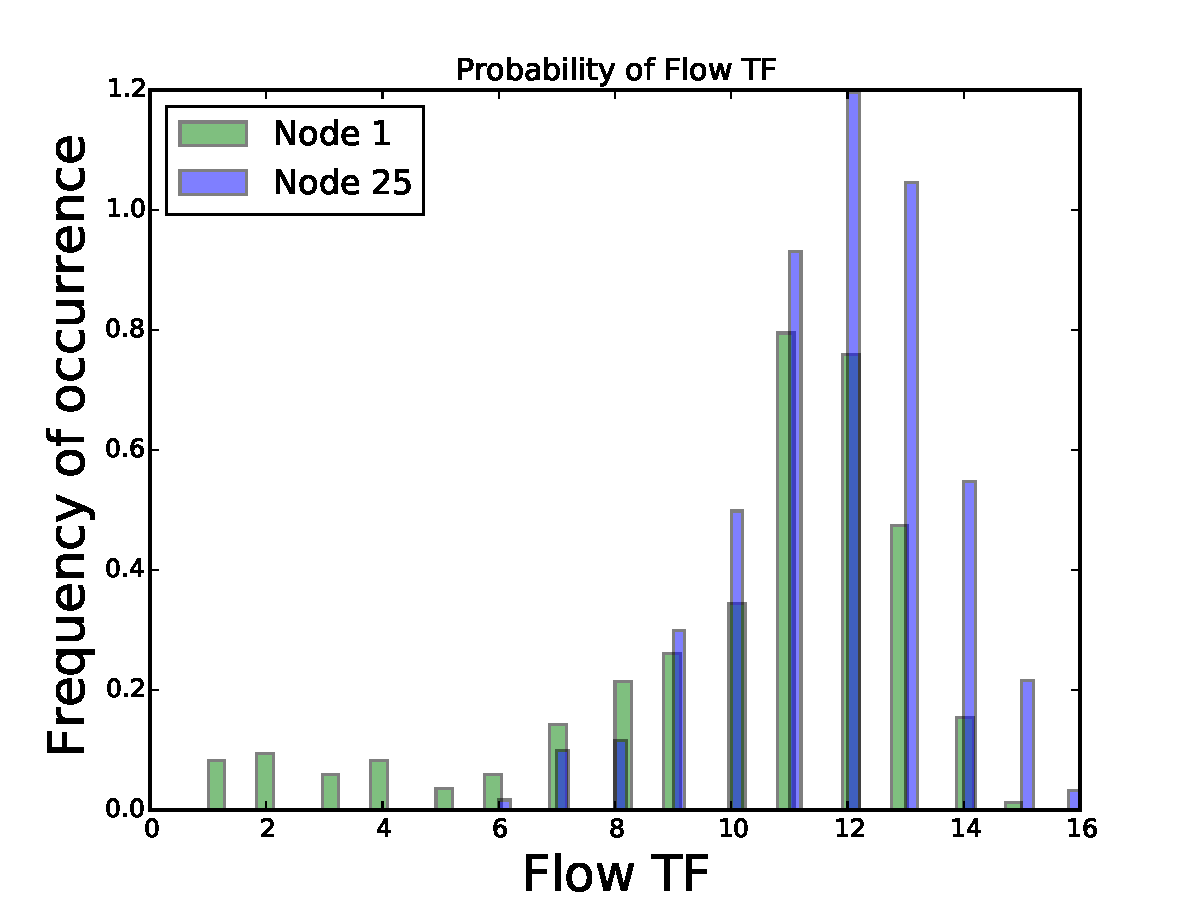
\includegraphics[scale=0.4, clip=true, trim=0mm 0mm 0mm 0mm]{figs_exp_vs_anal/num_nodes_50/image_size_360/timeliness_165/line_net/flow_TF_histogram.pdf}
    \caption{ Simulation results: Distribution of max TF of flows originating in the first node and the middle node in a line network with 50 nodes.  Image size = 360 KB}
    \label{fig:max_tf_dist_sim_N_50_IS_360}
\end{centering}
\end{figure}

I ran some simulations to see empirically what the actual maximum traffic factor is for flows.  Here, each node keeps track of the number of flows that it is currently forwarding, and every packet in each flow captures the maximum TF of any node along the path that it travels.  The result for flows originating in the first node in the line and the middle node in the line are plotted in \ref{fig:max_tf_dist_sim_N_50_IS_360}.  

\begin{figure}
\begin{centering}
	\subfigure[Analysis results: Distribution of expected maximum TF values for flows in the first and middle nodes using the derived TF expression in the other document]{
    		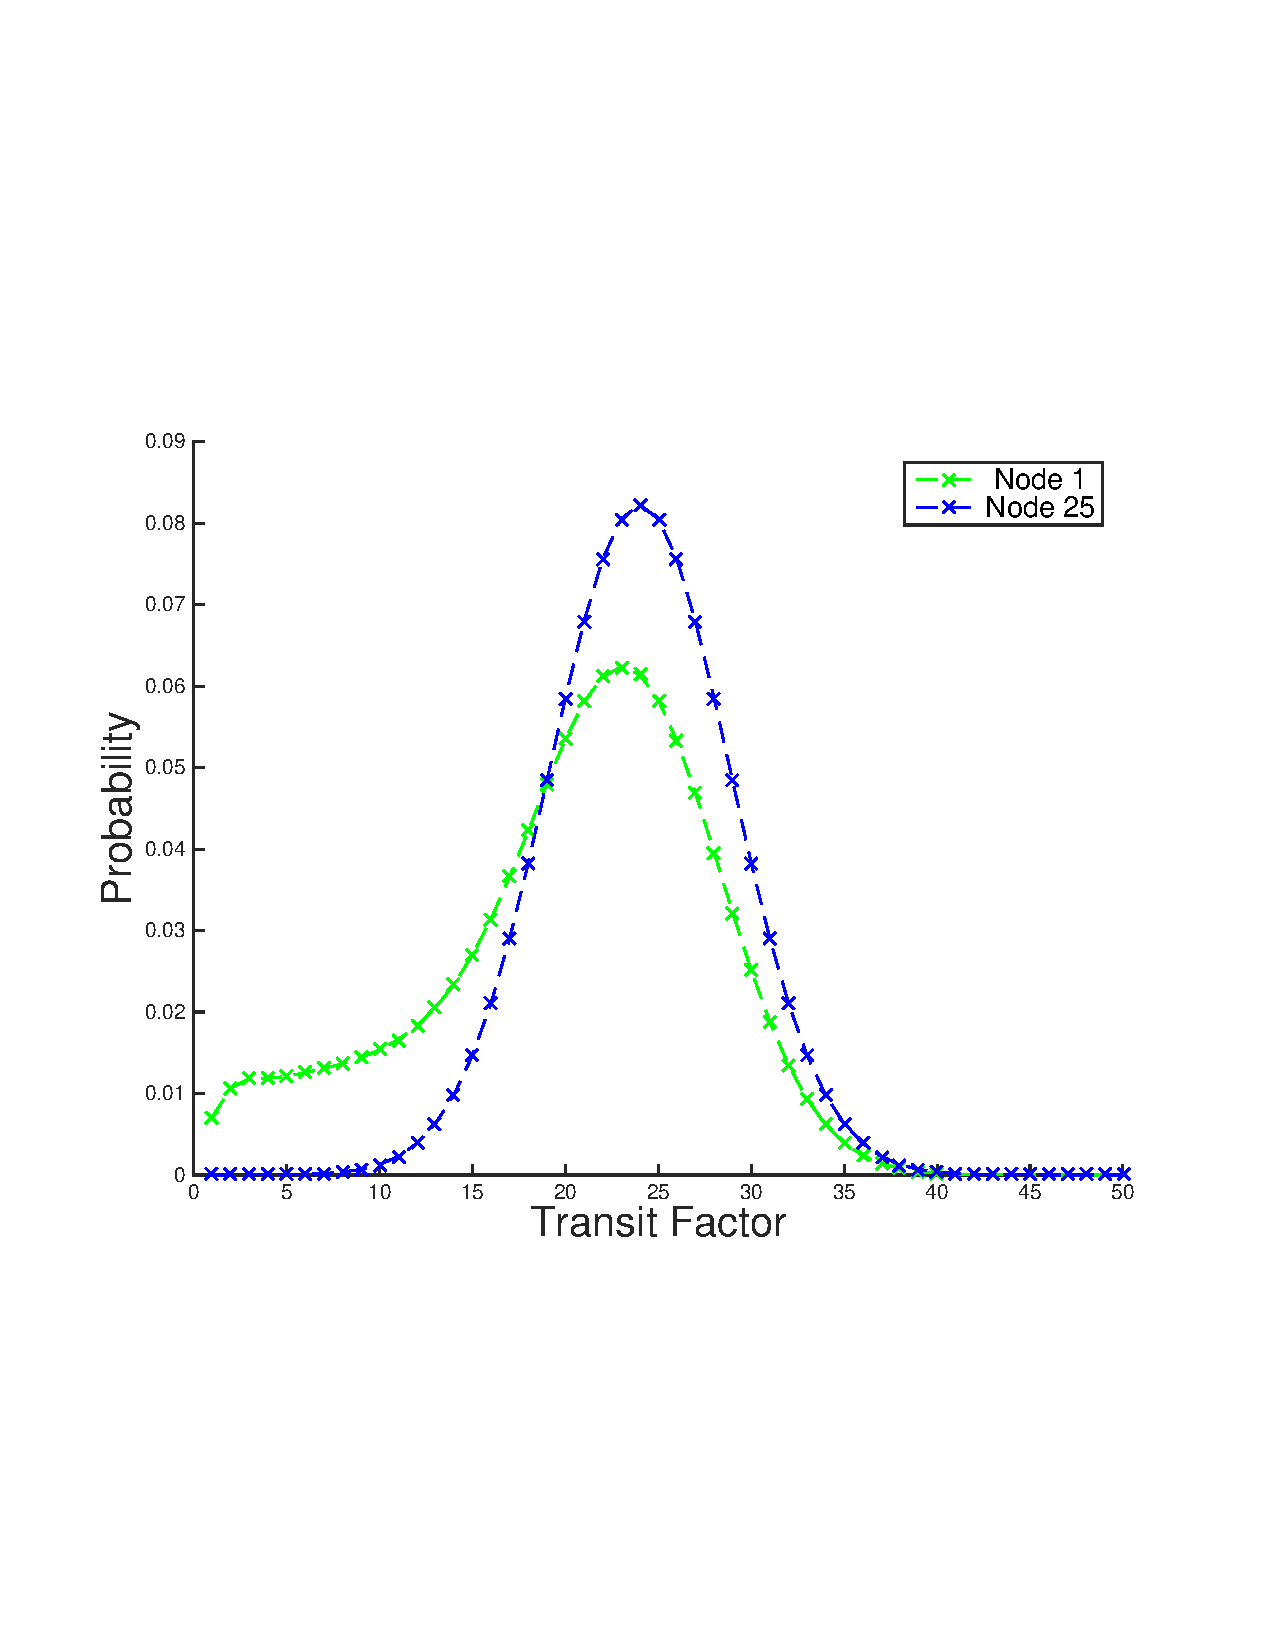
\includegraphics[scale=0.4, clip=true, trim=15mm 65mm 20mm 65mm]{figs_exp_vs_anal/num_nodes_50/image_size_360/timeliness_165/line_net/anal_flow_TF_pdf.pdf}
		\label{fig:max_tf_dist_anal_N_50_IS_360}
		}	
	\subfigure[Analysis results: Distribution of expected maximum TF values for flows in the first and middle nodes dividing the derived TF expression in the other document by 2]{
    		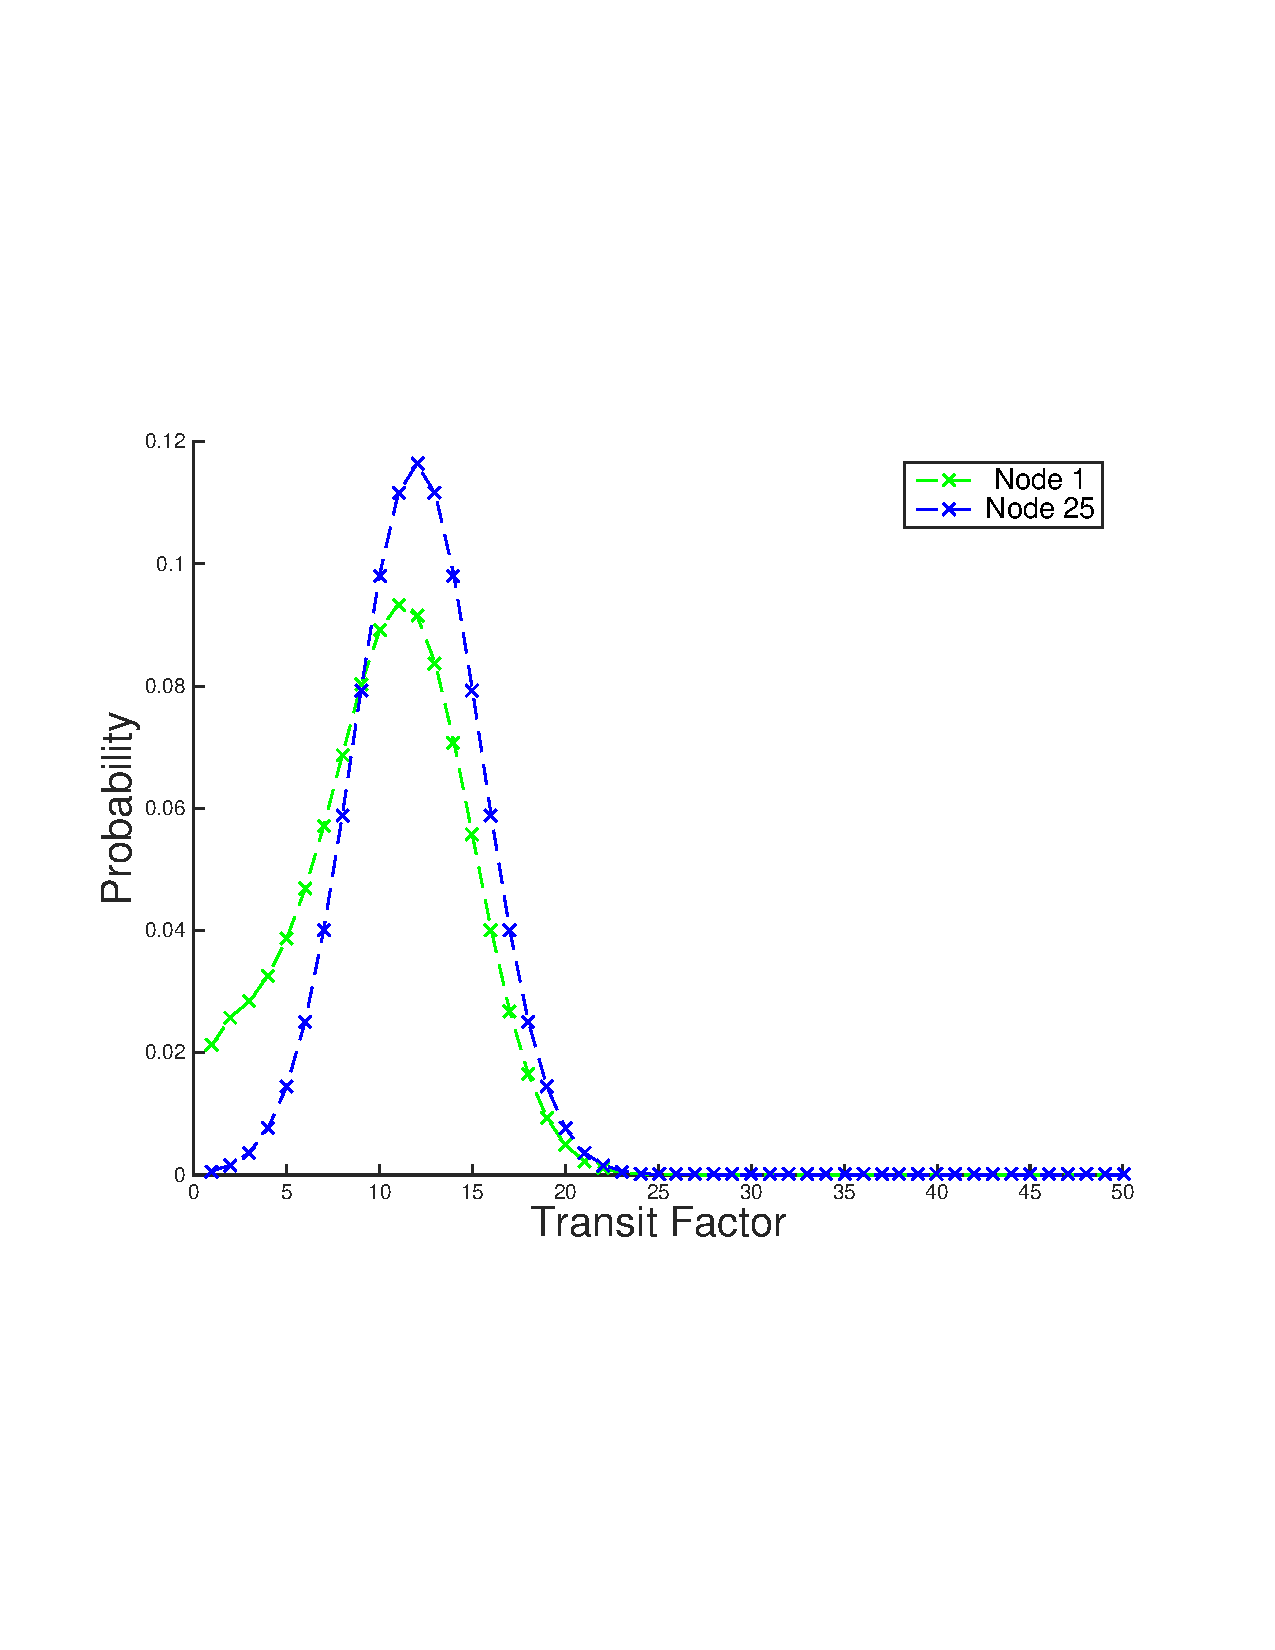
\includegraphics[scale=0.4, clip=true, trim=15mm 65mm 20mm 65mm]{figs_exp_vs_anal/num_nodes_50/image_size_360/timeliness_165/line_net/anal_flow_TF_pdf_2.pdf}
		\label{fig:max_tf_dist_anal_2_N_50_IS_360}
		}
	\caption{We can observe the empirical statistical properties of the Traffic Factor for each node's position in a line network (here with 125 nodes).}
	\label{fig:TF_empirical_stats_each_node_line_net}
\end{centering}
\end{figure}

In my working document of deriving the analytical model, I came up with the following expression for the expected TF in a node $x$:
\begin{equation}
	\frac{2 \cdot (x-1) \cdot (N-x)}{N-1}
\end{equation}
conditioning this expression on all possible destinations and the corresponding node with the max TF, we get the distributions for the TF of flows of the first and middle nodes plotted in Figure \ref{fig:max_tf_dist_anal_N_50_IS_360}.  Clearly, the mean value is much higher than what I was seeing in the simulations.  Interestingly enough, it seems that the mean values were about twice as high as I was seeing in simulations for several different network sizes, so I computed the distribution using the above expression divided by $2$.  That plot is in Figure \ref{fig:max_tf_dist_anal_2_N_50_IS_360}, which actually resembles the empirical results pretty well.  That leads me to my first question: Did I make a mistake in deriving an expression for TF that would have made it off by a factor of $2$?? 


\section{Delay}

I also collected and plotted a histogram of the delays that flows from each of the nodes experience in the simulations.  Figure \ref{fig:delay_dist_sim_N_50_IS_360} shows this distribution of delays for the same nodes again.  Here, we can see that the flows that experience the long delays are those that start in the end node.  This is not exactly the argument made in the WCNC paper, which accurately deduces that the maximum TF occurs at the center node, but also uses an average path length of $N/4$, which is for flows originating from the center node.  I'm actually still trying to reconcile why all of the results that use that formula were so accurate, but it seems that if we wrong on that equation, then it probably wasn't too far off because it does seem to be at least close. 

\begin{figure}
\begin{centering}
    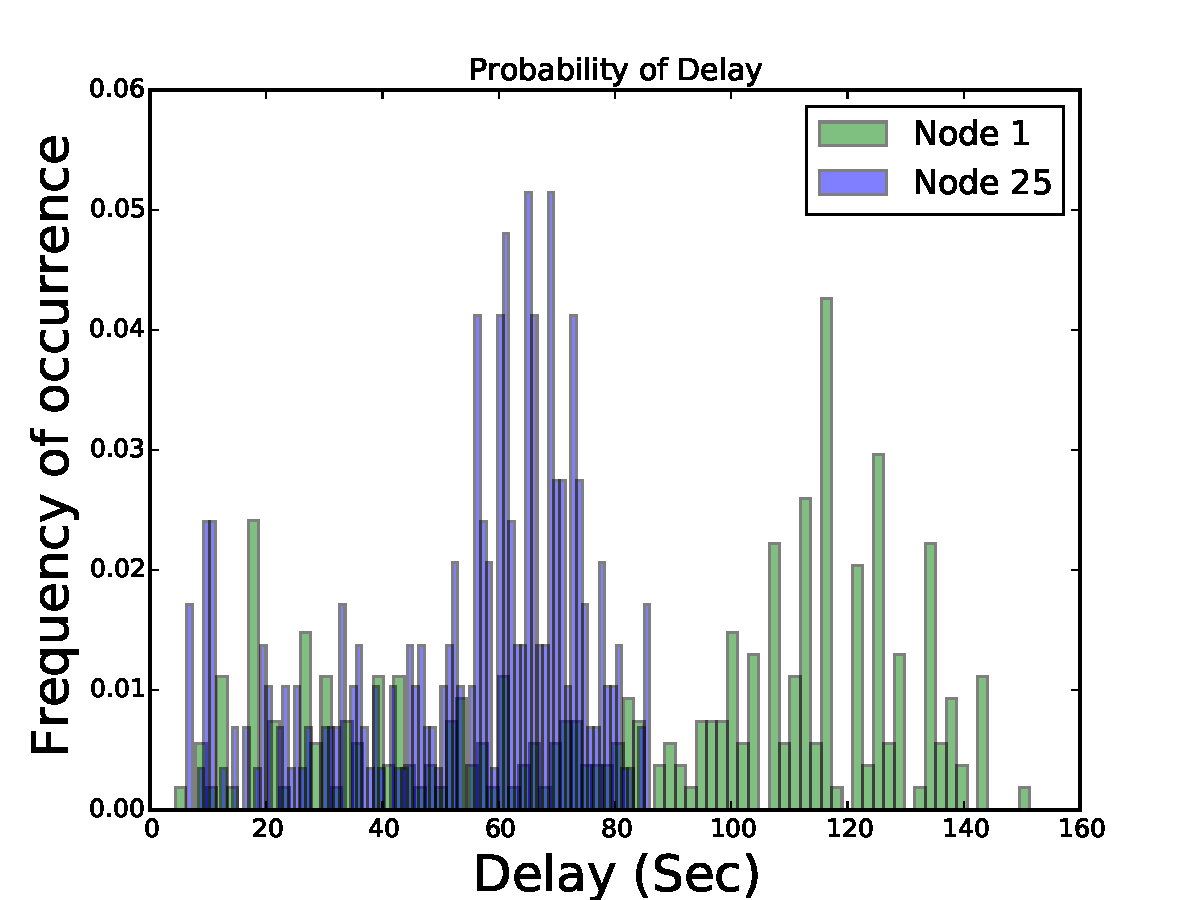
\includegraphics[scale=0.4, clip=true, trim=0mm 0mm 0mm 0mm]{figs_exp_vs_anal/num_nodes_50/image_size_360/timeliness_165/line_net/delay_histogram.pdf}
    \caption{ Simulation results: Distribution of delays of flows originating in the first node and the middle node in a line network with 50 nodes.  Image size = 360 KB}
    \label{fig:delay_dist_sim_N_50_IS_360}
\end{centering}
\end{figure}

Coming back to the formulation of a delay distribution, though, I also computed and plotted analytical values of the derived model.  First, if I use the derived expressions from the other document, including the expression for TF that seems to have a mean twice as large as the empirical values, the delays don't seem correct.  They are not always close to ending around the maximum delays observed in simulations, and they don't project the flows from node $1$ having higher delay than those of the middle node.  To provide an example, I plotted this case in Figure \ref{fig:max_tf_dist_anal_N_50_IS_360}.

So, I first tried using the distribution of TFs that is closer to the simulation results (in Figure \ref{fig:max_tf_dist_anal_2_N_50_IS_360}), but that doesn't provide matching distributions, because the flows from node $1$ do not exceed the center node as seen in the simulations.  It seems that path lenght has a larger impact on delays than what I had previously formulated (more evidence of this in Figure \ref{fig:pl_vs_delay_scatter_N_50_IS_360})...so I started playing with the factors.  For a few scenarios, multiplying the second portion of the delay, i.e., the multi-hop propagation portion, by a factor proportional to the number of packets in a flow seems to be close(r).  Figure \ref{fig:max_tf_dist_anal_2_N_50_IS_360} calculates the delay distribution using the original TF expression divided $2$ and multiplying the $C_2 \cdot PL(i,j)$ part of the delay by $\frac{P_n}{2}$, where $P_n$ is the number of packets in a flow.  

In the WCNC paper, I argue that this delay is only experienced once per flow, and, thus, should not be multiplied by this extra factor, but I'm wondering if that also isn't quite accurate??  I'm still trying to run more simulations and trace more closely what is happening to figure out where the discrepancies are and what is causing them.

\begin{figure}
\begin{centering}
	\subfigure[Analysis results: Distribution of delay values for flows in the first and middle nodes using the derived TF expression in the other document]{
    		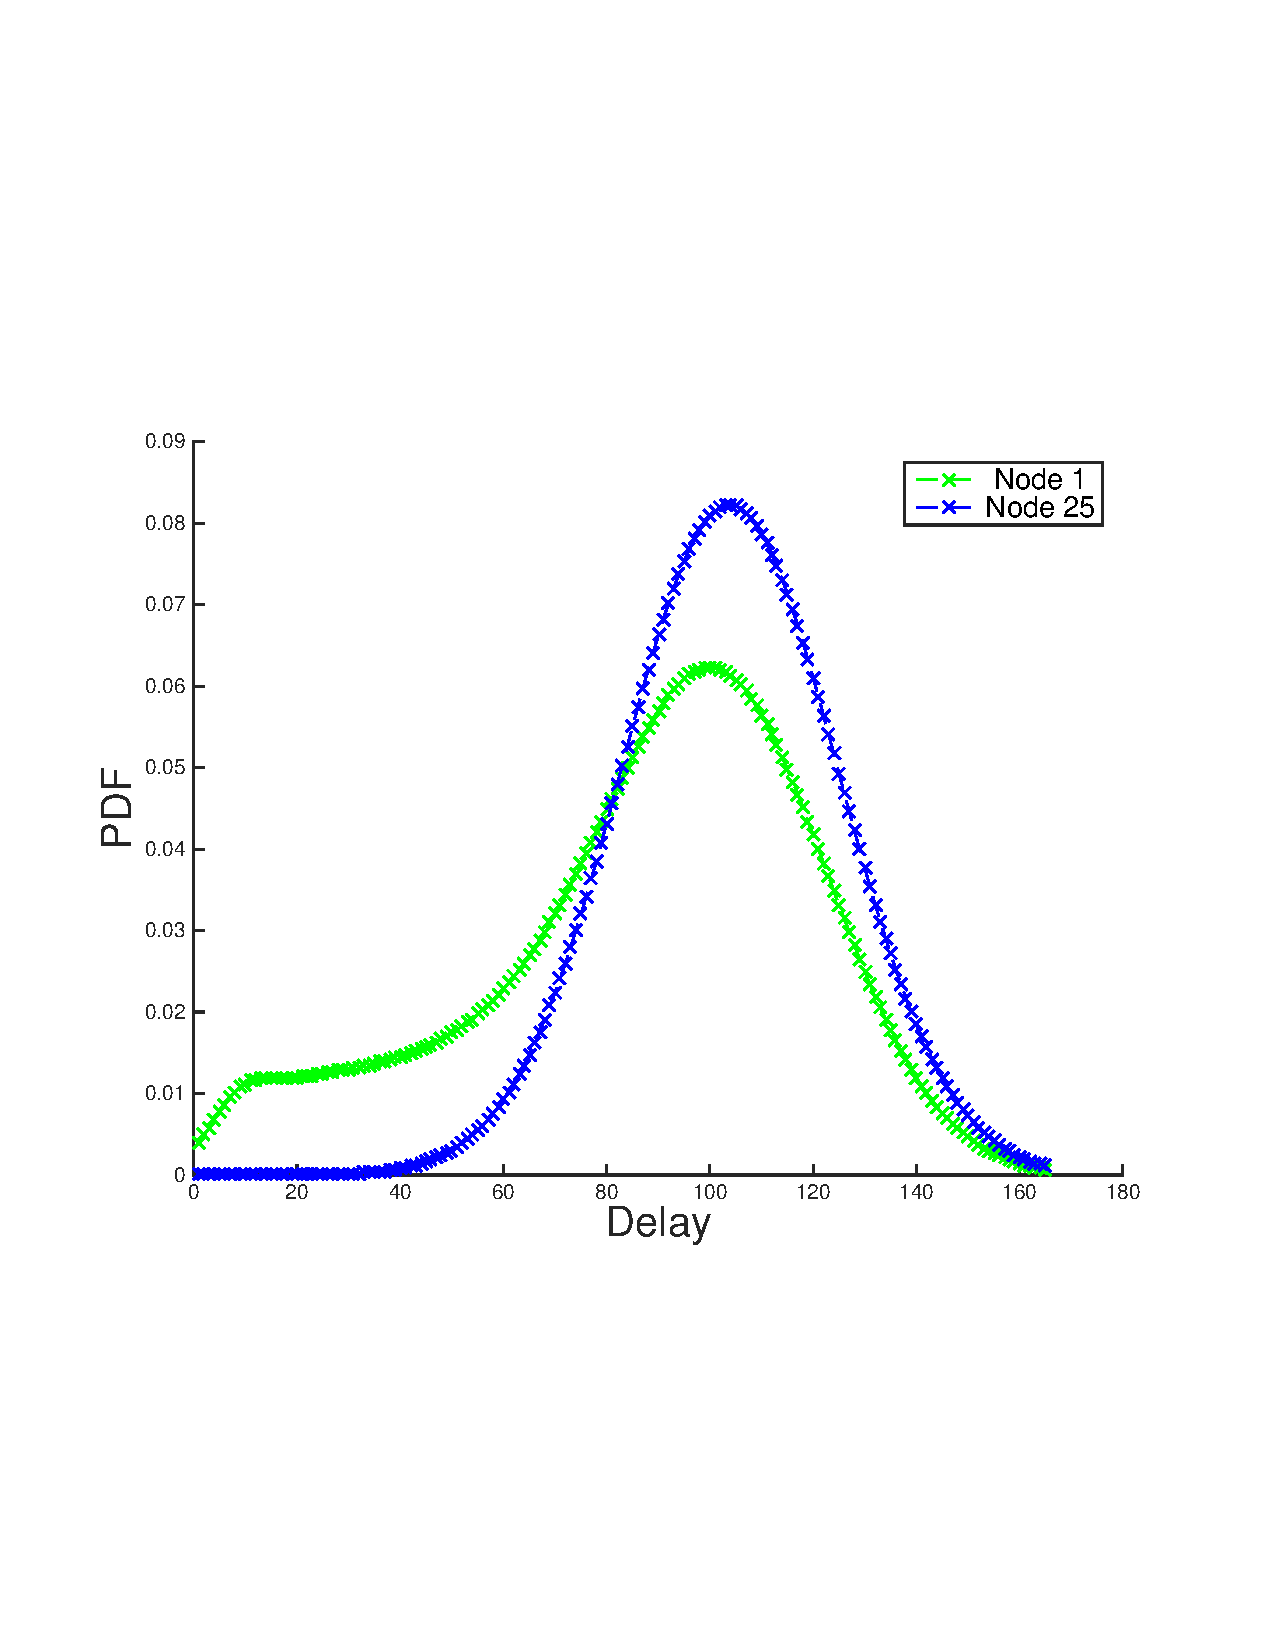
\includegraphics[scale=0.4, clip=true, trim=15mm 65mm 20mm 65mm]{figs_exp_vs_anal/num_nodes_50/image_size_360/timeliness_165/line_net/anal_delay_pdf_1.pdf}
		\label{fig:delay_dist_anal_N_50_IS_360}
		}	
	\subfigure[Analysis results: Distribution of delay values for flows in the first and middle nodes dividing the derived TF expression in the other document by 2]{
    		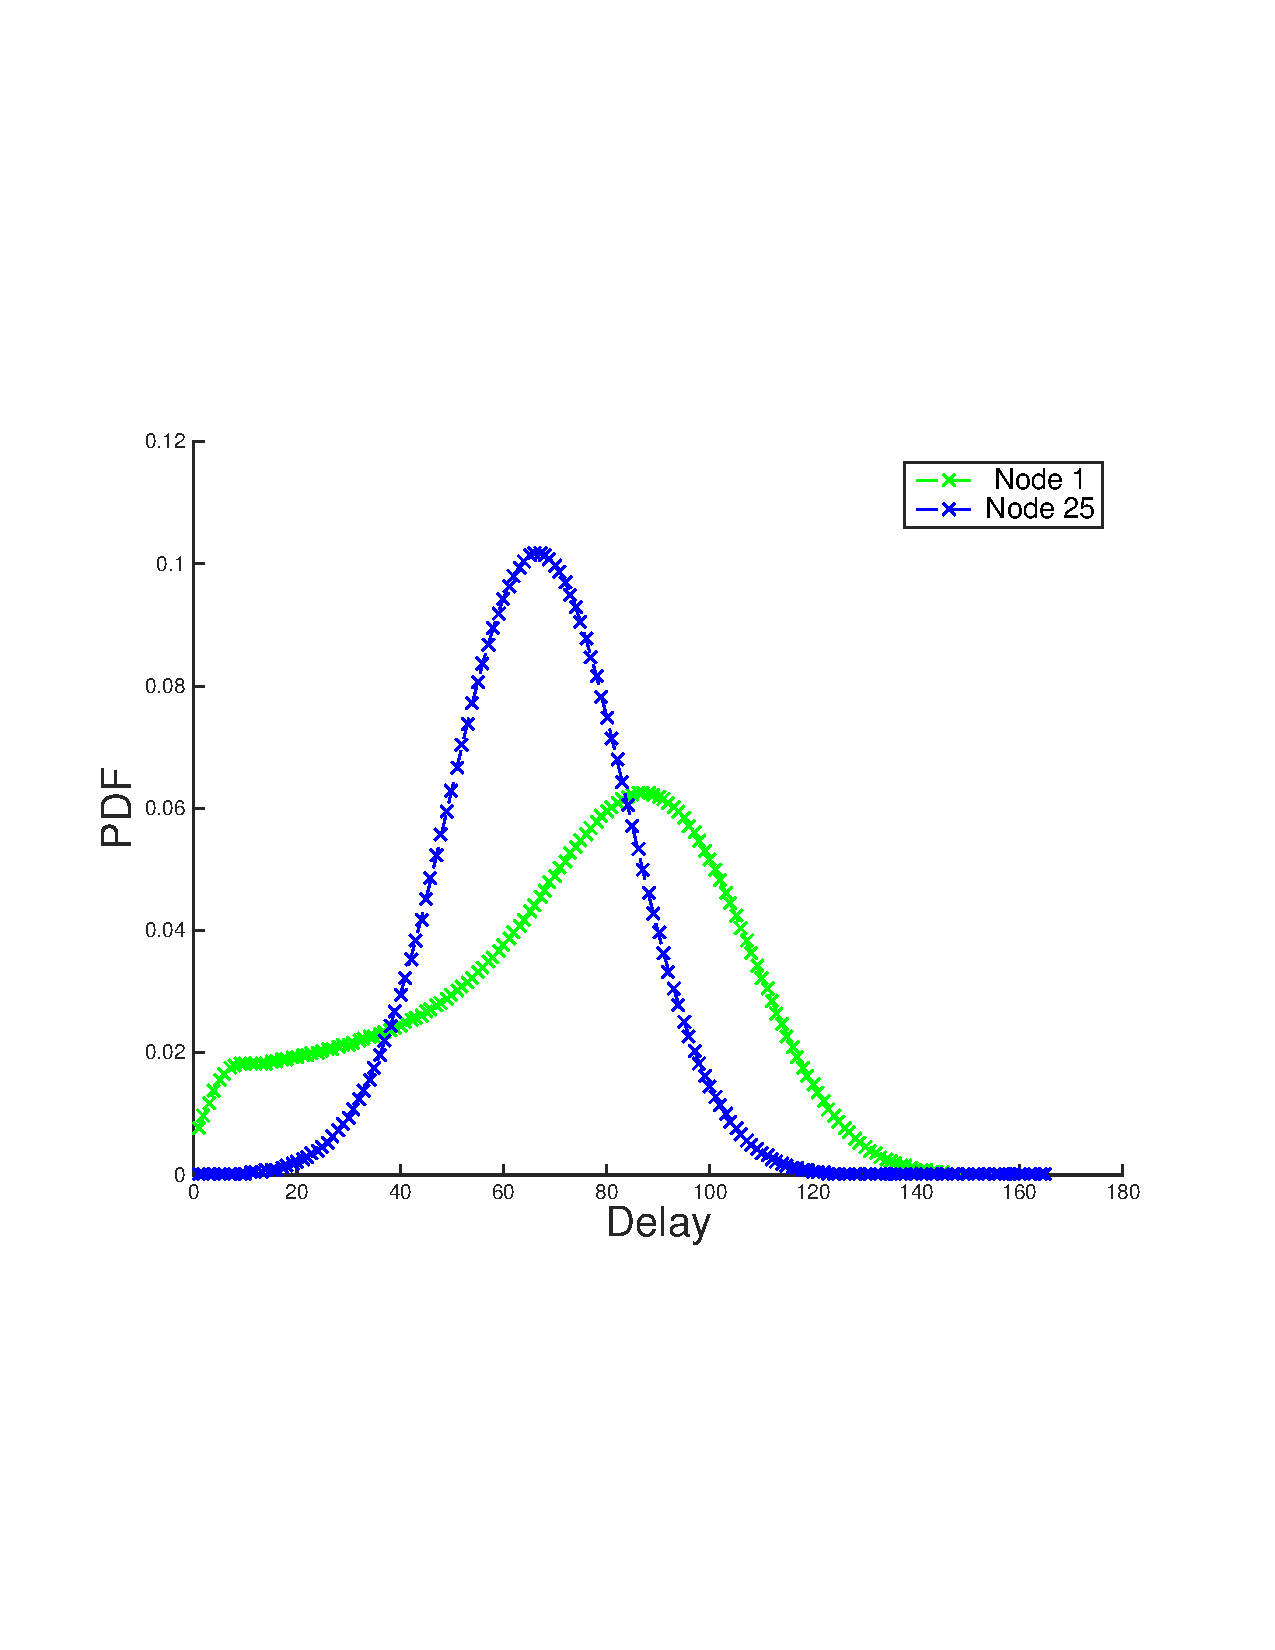
\includegraphics[scale=0.4, clip=true, trim=15mm 65mm 20mm 65mm]{figs_exp_vs_anal/num_nodes_50/image_size_360/timeliness_165/line_net/anal_delay_pdf_2.pdf}
		\label{fig:delay_dist_anal_2_N_50_IS_360}
		}
	\caption{We can observe the empirical statistical properties of the Traffic Factor for each node's position in a line network (here with 125 nodes).}
	\label{fig:TF_empirical_stats_each_node_line_net}
\end{centering}
\end{figure}

\section{Other Simulation Results}

Some other things that I tracked in simulations and plotted provide some insight, too.  First, I modified the original stochastic expression of delay because I realized that the Traffic Factor and path length are not really independent.  If you think about a flow beginning in node $1$, this makes sense since the max TF of the flow depends exactly on what the destination is.  Figure \ref{fig:pl_vs_tf_scatter_N_50_IS_360} shows a scatter plot of the max TF experienced by each flow given its path length.  Flows beginning in the center node are pretty evenly distributed and appear to be somewhat independent of path length.  The flows beginning in node $1$, though, have a linear dependence on path length until it reaches about half of the network size, at which point it levels off and is evenly distributed independently for path lengths to the full length of the network.  

\begin{figure}
\begin{centering}
    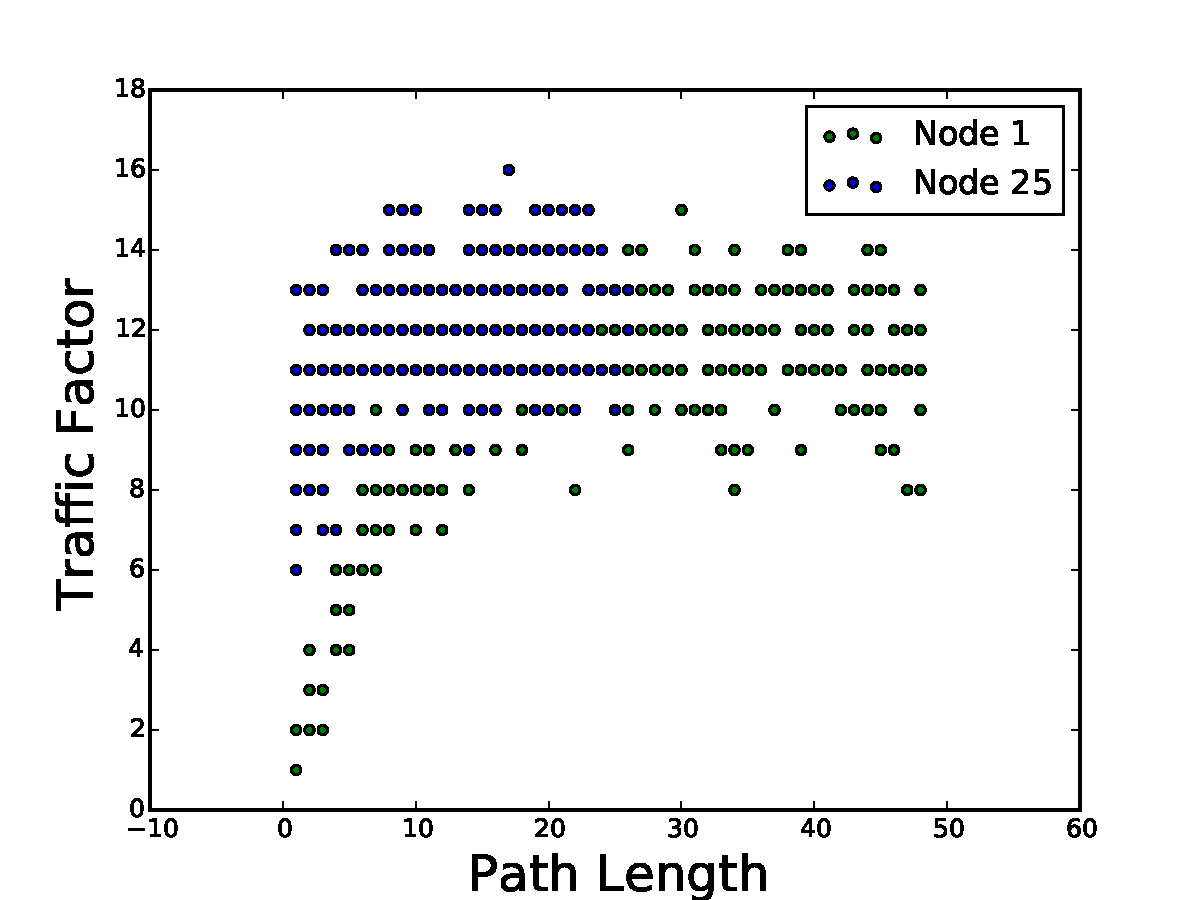
\includegraphics[scale=0.4, clip=true, trim=0mm 0mm 0mm 0mm]{figs_exp_vs_anal/num_nodes_50/image_size_360/timeliness_165/line_net/PL_vs_TF_scatter.pdf}
    \caption{ Simulation results: Scatter of TF vs. Path Length for flows in the first node and the middle node in a line network with 50 nodes.  Image size = 360 KB}
    \label{fig:pl_vs_tf_scatter_N_50_IS_360}
\end{centering}
\end{figure}

As I stated earlier, it seems that the path length has a larger impact on overall delay than I had accounted for previously.  This seems to be reinforced by plotting the delay vs. path length of flows in Figure \ref{fig:delay_vs_PL_scatter_N_50_IS_360}.  The trend is pretty clearly linear.  I also plotted the delay vs. traffic factor values in Figure \ref{fig:delay_vs_TF_scatter_N_50_IS_360}.  This relationship also seems to be linear, but more spread.  Since I believe that path length and traffic factor are not independent, I'm not exactly sure how to interpret these results, but I think it might point to a larger scaling factor for the multi-hop propagation component of delay than we originally surmised.  

\begin{figure}
\begin{centering}
    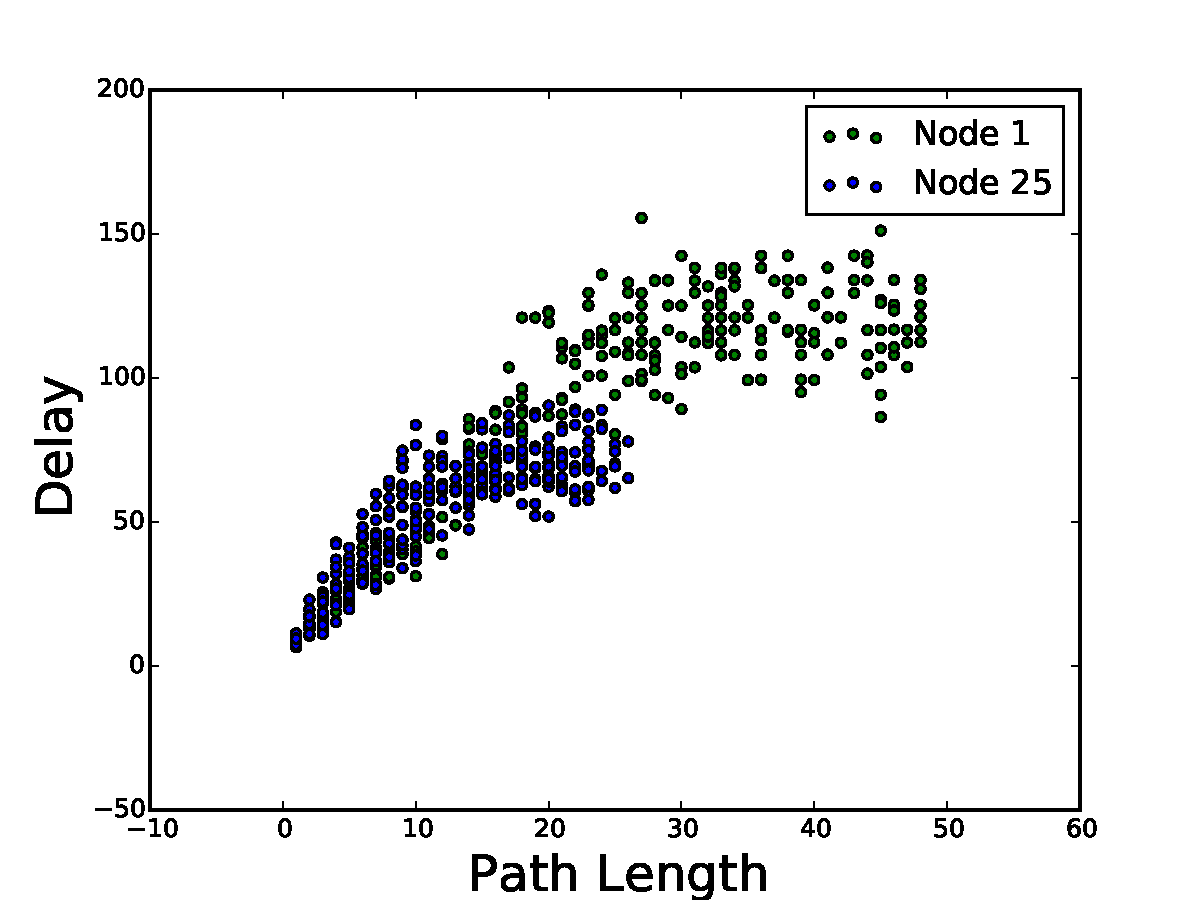
\includegraphics[scale=0.4, clip=true, trim=0mm 0mm 0mm 0mm]{figs_exp_vs_anal/num_nodes_50/image_size_360/timeliness_165/line_net/delay_vs_PL_scatter.pdf}
    \caption{ Simulation results: Scatter of delay vs. Path Length for flows in the first node and the middle node in a line network with 50 nodes.  Image size = 360 KB}
    \label{fig:delay_vs_PL_scatter_N_50_IS_360}
\end{centering}
\end{figure}

\begin{figure}
\begin{centering}
    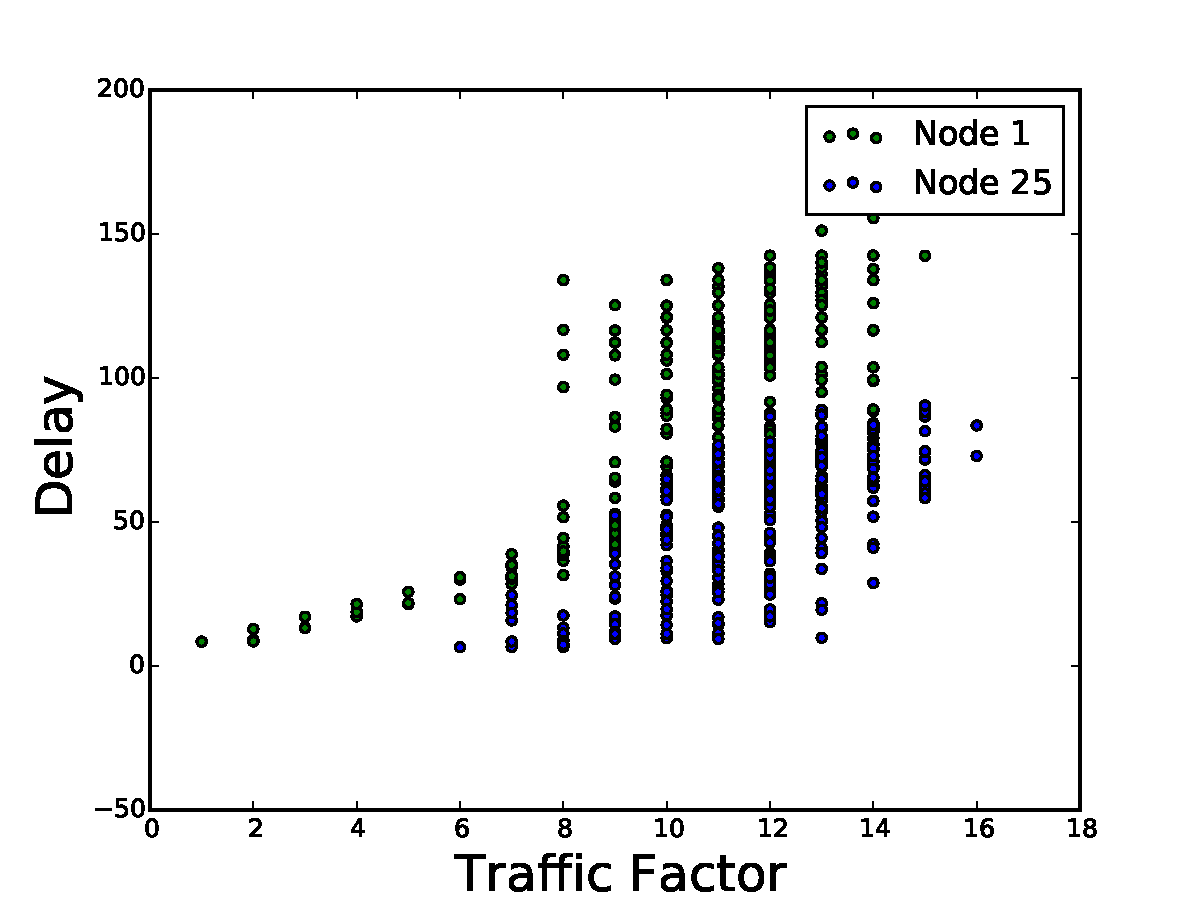
\includegraphics[scale=0.4, clip=true, trim=0mm 0mm 0mm 0mm]{figs_exp_vs_anal/num_nodes_50/image_size_360/timeliness_165/line_net/delay_vs_TF_scatter.pdf}
    \caption{ Simulation results: Scatter of delay vs. max Traffic Factor for flows in the first node and the middle node in a line network with 50 nodes.  Image size = 360 KB}
    \label{fig:delay_vs_TF_scatter_N_50_IS_360}
\end{centering}
\end{figure}

%\appendix
%\input{sections/random_explanation}
% conference papers do not normally have an appendix


% use section* for acknowledgement
%\section*{Acknowledgment}


%The authors would like to thank...


% trigger a \newpage just before the given reference
% number - used to balance the columns on the last page
% adjust value as needed - may need to be readjusted if
% the document is modified later
%\IEEEtriggeratref{8}
% The "triggered" command can be changed if desired:
%\IEEEtriggercmd{\enlargethispage{-5in}}

% references section

% can use a bibliography generated by BibTeX as a .bbl file
% BibTeX documentation can be easily obtained at:
% http://www.ctan.org/tex-archive/biblio/bibtex/contrib/doc/
% The IEEEtran BibTeX style support page is at:
% http://www.michaelshell.org/tex/ieeetran/bibtex/
%\bibliographystyle{IEEEtran}
% argument is your BibTeX string definitions and bibliography database(s)
%\bibliography{IEEEabrv,../bib/paper}
%
% <OR> manually copy in the resultant .bbl file
% set second argument of \begin to the number of references
% (used to reserve space for the reference number labels box)
%\begin{thebibliography}{1}


\bibliographystyle{unsrt}

\bibliography{references}

%\bibitem{IEEEhowto:kopka}
%H.~Kopka and P.~W. Daly, \emph{A Guide to \LaTeX}, 3rd~ed.\hskip 1em plus
%  0.5em minus 0.4em\relax Harlow, England: Addison-Wesley, 1999.

%\end{thebibliography}




% that's all folks
\end{document}


